%!TEX root=../document.tex

\section{Einführung}

Schreiben Sie zu die Klasse Bruch in einem Modul bruch

Nutzen Sie die Testklassen  in PyCharm.

Ziel: Coverage > 95\%

\subsection{Aufgabenstellung}

Empfohlene Vorgehensweise:

    Projekt in PyCharm erstellen
    Modul bruch erstellen
    Klasse Bruch erstellen
    Test-Ordner erstellen
    Unit-Tests entpacken und lauffähig machen

Abgabe:

Protokoll mit Testreports (inkl. Coverage) und Dokumentation (html)

Abgabe des Python-files

Achtung: Vergessen Sie nicht auf eine ausführliche Dokumentation mittels sphinx

%Listen erstellen
%\begin{itemize}
%	\item \textbf{ \"Ubungsteil 1:} 
%	\item \textbf{ \"Ubungsteil 2: } 
%\end{itemize}

%Bilder einfügen
%\begin{figure}[!h]
%	\begin{center}
%		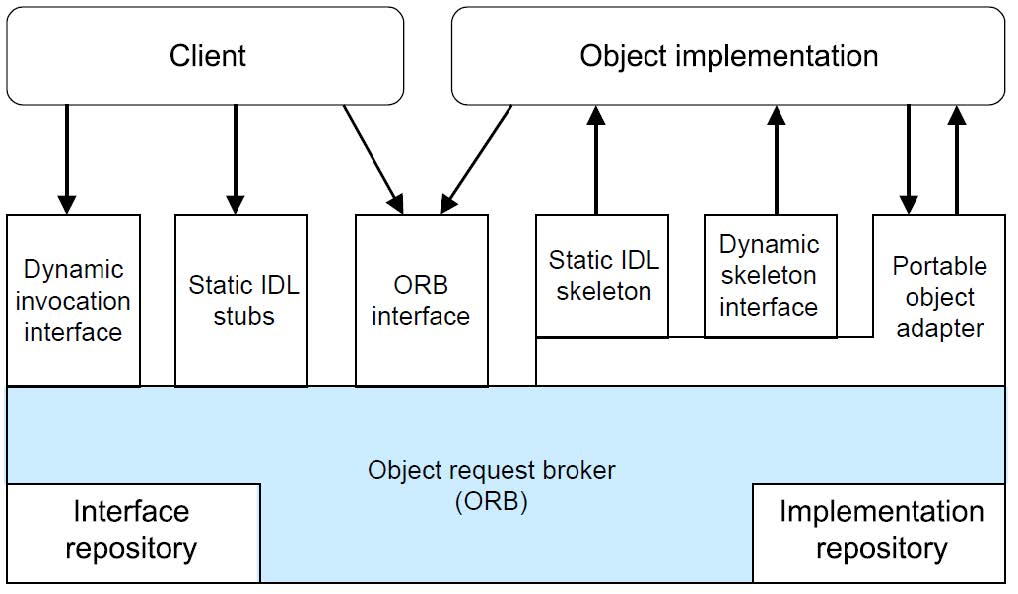
\includegraphics[width=0.5\linewidth]{images/corba.jpg}
%		\caption{Common Object-Request-Broker Architecture \cite{tanenbaum2007verteilte}}
%		\label{broker}
%	\end{center}
%\end{figure}
%
\clearpage
